\documentclass{article}
\usepackage[utf8]{inputenc}
\usepackage{amssymb}
\usepackage{graphicx}
\usepackage{geometry}

% Don't print section numbers
\setcounter{secnumdepth}{0}

% Turn off header and footer
\pagestyle{empty}

%Tabulatoreinstellungen
\newcommand\tab[1][1cm]{\hspace*{#1}}

%Seiteneinstellungen
\geometry{top=2cm,bottom=1cm}

%-----------------------------------------------------

\begin{document}

\section{RSA-Algorithmus}

\fbox{privater Schlüssel: a}
\fbox{öffentlicher Schlüssel: n und b}

\subsection{1. Zwei Primzahlen wählen + Produkt berechnen}
\(p = 11, q = 19\) \tab \(n= p \cdot q = 209\)

\subsection{2. Satz von Euler \(\varphi (n)\)}
Wird für 3. benötigt
\(\varphi(n) = \varphi(p \cdot q) = \varphi(p) \cdot \varphi (q) = (p -1)(q-1)\)\\
\(\varphi(209) = \varphi(11) \cdot \varphi(19) = 10 \cdot 18 = 180\)

\subsection{3. Private Key bestimmen, Zahl \(a\) suchen}
Bedingungen:
\begin{itemize}
    \item \(0\leq a<\varphi(n)\)
    \item \(ggT(\varphi(n),a)=1\)
\end{itemize}
\(ggT(180, 101) = 1\)\\
\fbox{privater Schlüssel: \(a=101\)}

\subsection{öffentlicher Schlüssel vervollständigen, \(b\) bestimmen}
Das multiplikative Inverse von \(a\) in \(\mathbb{Z}_{\varphi(n)}\) ist gesucht\\
Erweiterter euklidischer Algorithmus verwenden\\
\(t = b\)\\
\(ggT(\varphi(n),a) = 1 \rightarrow t \cdot a \equiv 1 mod \varphi(n)\)\\ \\
\(a^{-1}\) in \(\mathbb{Z}_{180}\):\\
\begin{tabular}{cccc|cccc}
    x & y & q & r &  u & s & v & t\\
    180 & 101 & 1 & 79 & 1 & 0 & 0 & 1\\
     101 & 79 & 1 & 22 &  0 & 0 & 1 & -1\\
     79 & 22 & 3 & 13 &  0 & 0 & -1 & 2\\
     22 & 13 & 1 & 9 & 0 & 0 & 2 & -7\\
     13 & 9 & 1 & 4 & 0 & 0 & -7 & 9\\
     9 & 4 & 2 & 1 & 0 & 0 & 9 & -16\\
     4 & 1 & 4 & 0 & 0 & 0 & -16 & \textbf{41}
\end{tabular}\\ \\
\fbox{öffentlicher Schlüssel: \(n=209, b=41\)}

\section{Verschlüsseln/Entschlüsseln}
Verschlüsseln: \(d=c^{b} mod n\) Entschlüsseln \(e \equiv d^{a} mod n\)\\
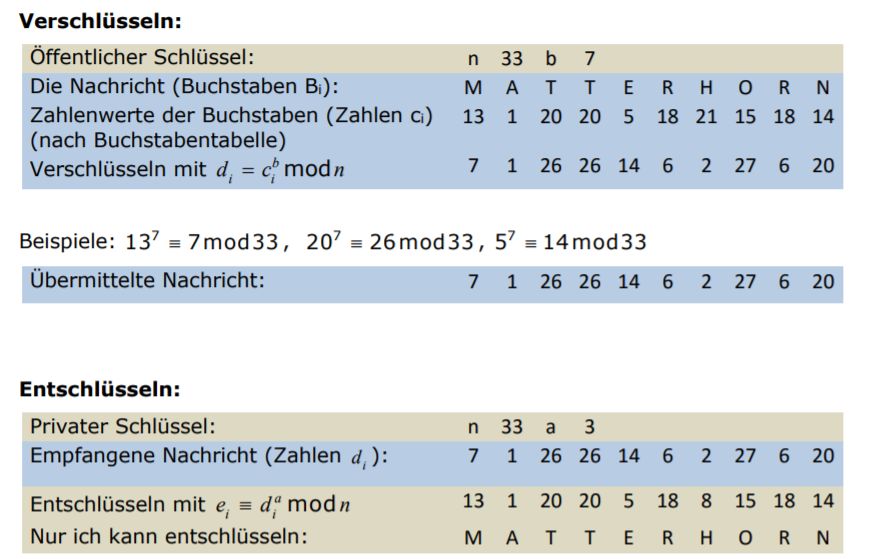
\includegraphics[scale=.5]{rsa.PNG}

\end{document}
